\section{Úchovávání dat}

Jak již bylo zmíněno, uživatelská data a samotná aplikace musí být někde uchovávány. Webová aplikace (tj. VueJS frontend a Laravel backend) je nasazena pomocí služby "App Platform" od poskytovatele DigitalOcean. PostgreSQL databáze pro administraci nad uživatelskými daty a formuláři, jejíž struktura bude rozebrána v této části, je nasazena na Heroku serveru. 

\subsection{Struktura databáze}
K tomu, aby byla struktura databáze vysvětlena, je níže vygenerováno schéma, které by mělo sloužit pro lepší vizualizaci.

\begin{figure}[h]
	\centering %% příkaz, který ti obrázek zarovná na střed
	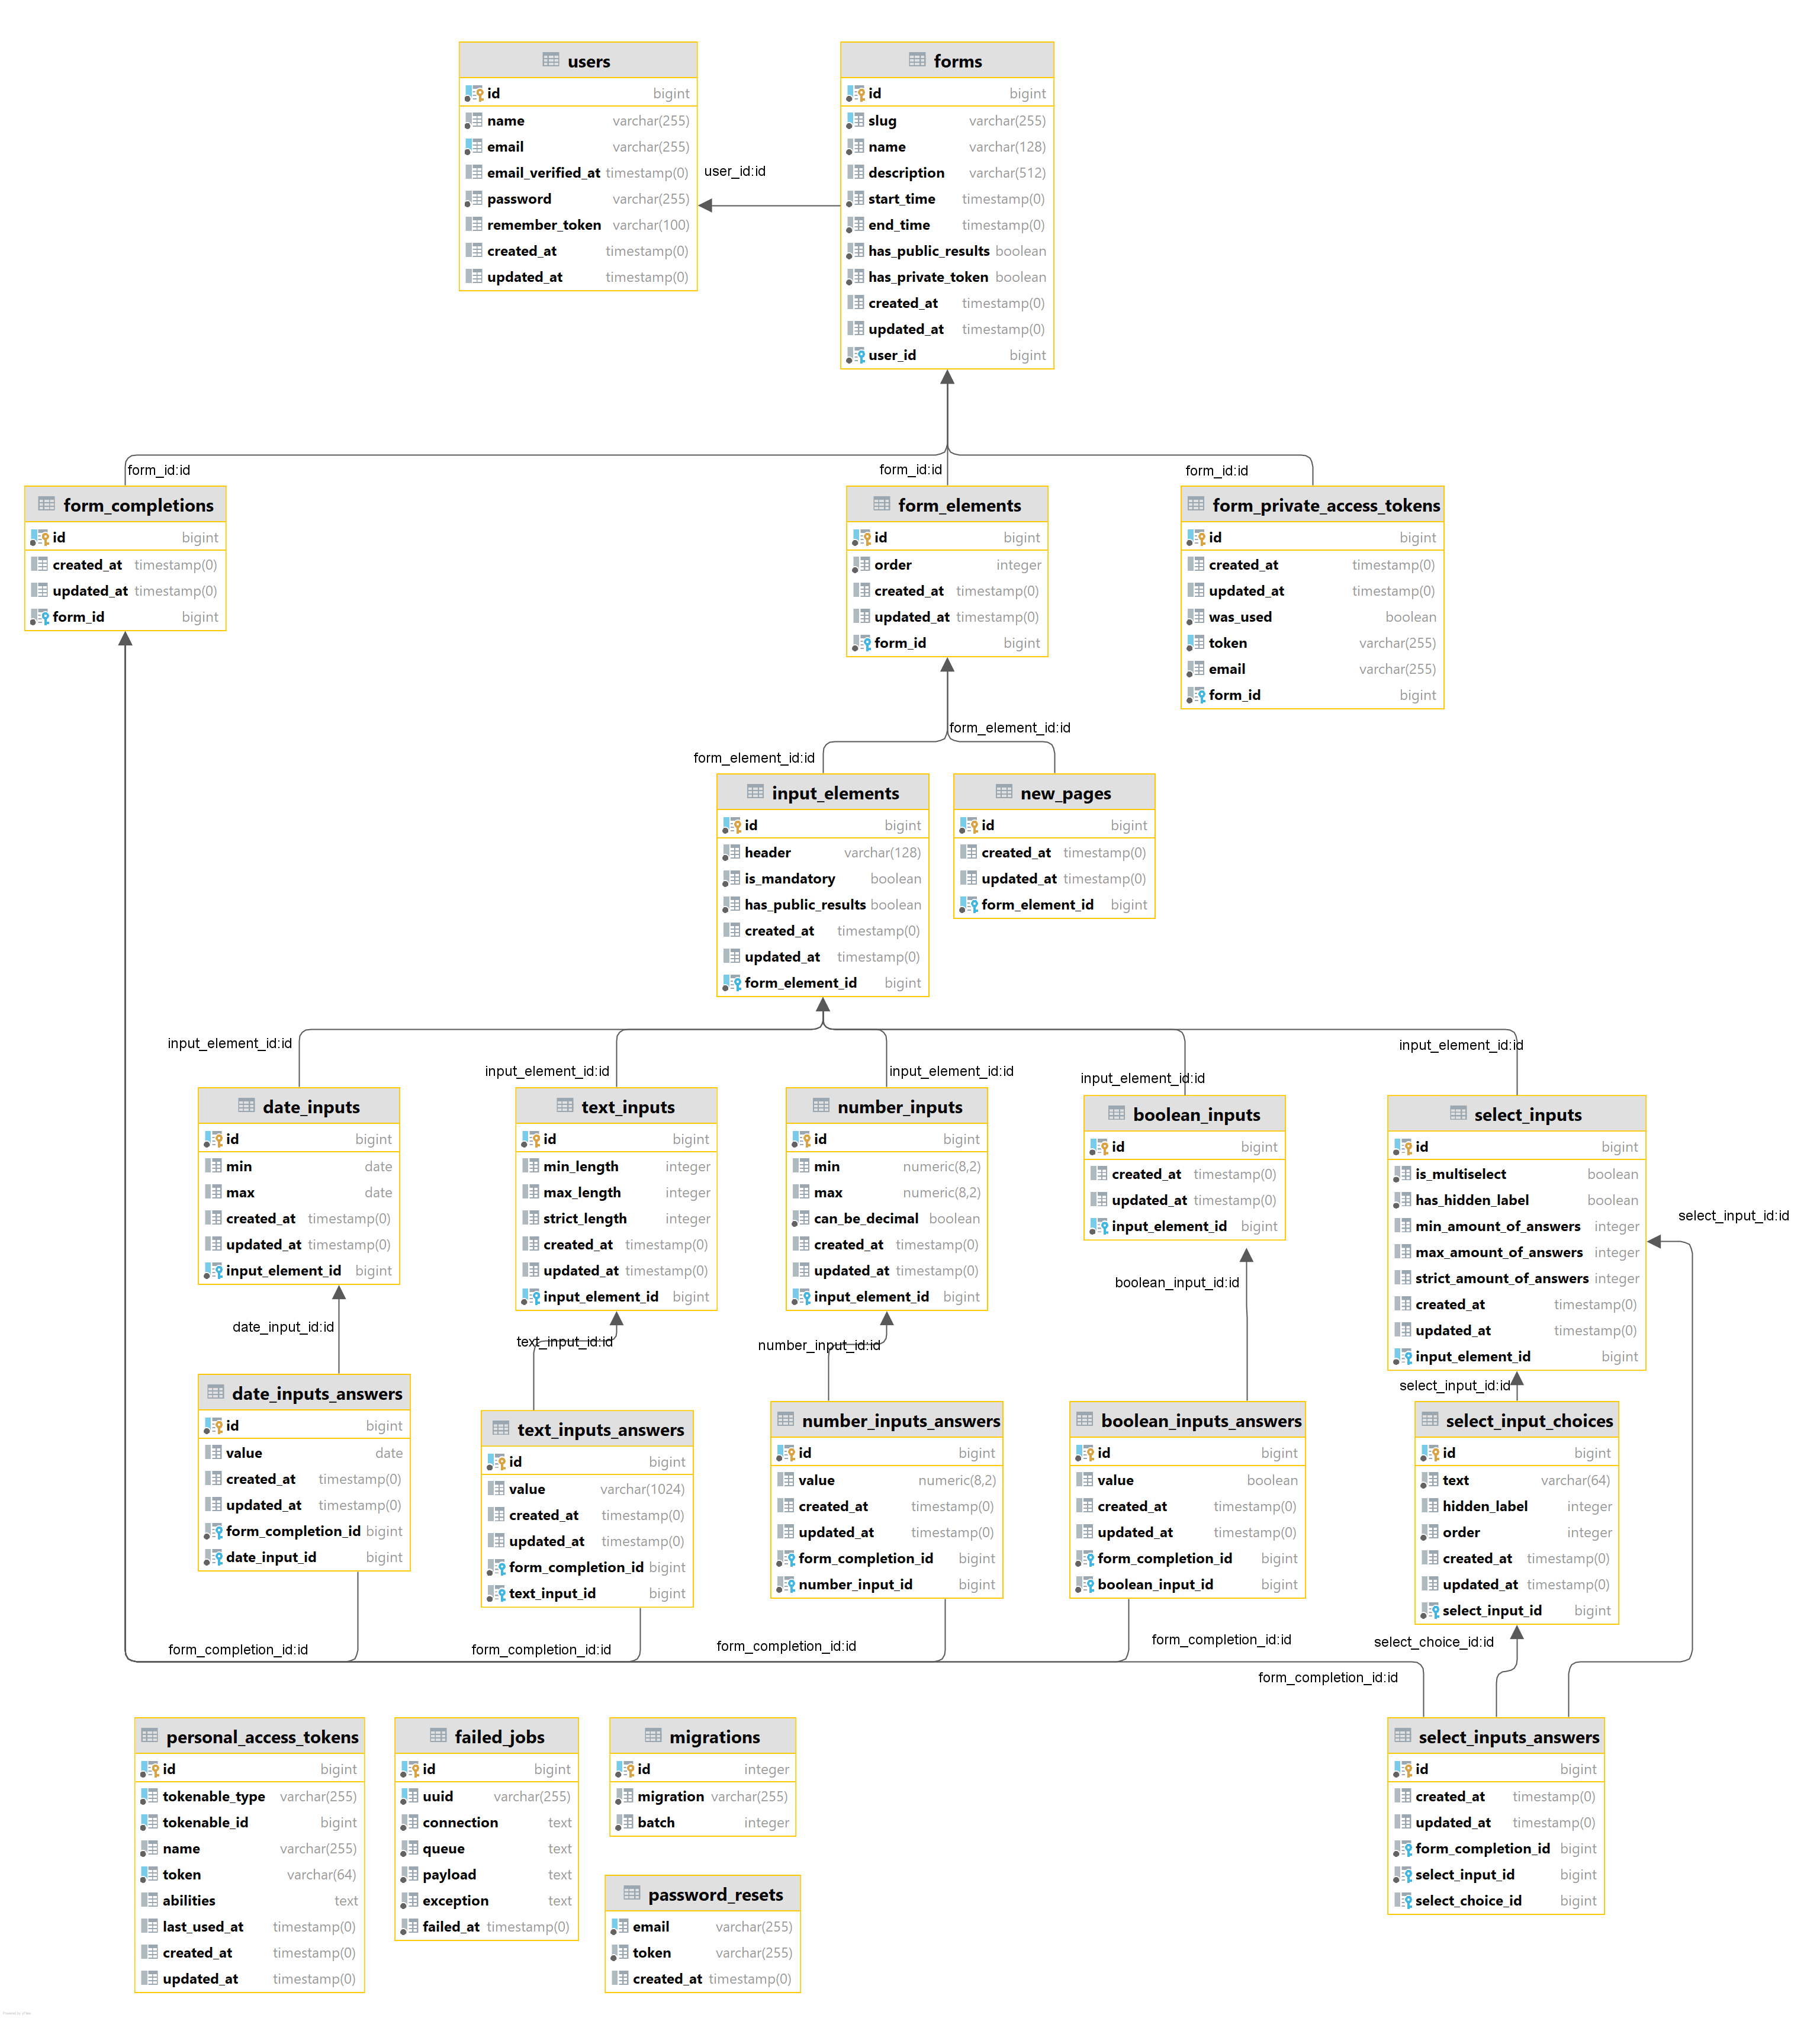
\includegraphics[width=0.6\textwidth]{img/db_diagram.png} %% vložení samotného obrátku
	\caption{Diagram struktury databáze vygenerovaný aplikací DataGrip !!!citace!!!} %% popisek obrázku, nezapomeň na citace!
	\label{fig:db_diagram} %% označení až budeš chtít na obrázek odkazovat
\end{figure}

Jak je již z obrázku vidět, databáze je tvořena tabulkami, které jsou provázány určitými relacemi. Všechny tabulky mají unikátní primární klíč (ve všech tabulkách kromě \textit{password\_resets} atribut \textit{id}), kterým lze identifikovat jednotlivé instance. Většina z nich má také tzv. cizí klíč, který slouží k propojení s jinou tabulkou na základě shody tohoto klíče s cizím primárním klíčem. Také většina obsahuje předgenerované atributy timestamps (v překladu časová razítka) \textit{created\_at} a \textit{updated\_at}, které nám umožňují sledovat, kdy byla položka vytvořena či upravena.

Základním objektem databáze je samotný uživatel (tabulka \textit{users}), který obsahuje standardní vlastnosti jako jsou: uživatelské jméno (\textit{name}), emailovou adresu (\textit{email}), která také slouží jako identifikátor (musí být unikátní), heslo v zašifrované podobě (\textit{password}) a další předgenerované atributy, které jsou využívány primárně samotným frameworkem Laravel.

Dalším důležitým základním objektem je formulář (tabulka \textit{forms}). Tento objekt reprezentuje samotný dotazník a jeho vlastnosti.

%databázové objekty a jejich vlastnosti